\documentclass[conference]{IEEEtran}
\IEEEoverridecommandlockouts
% The preceding line is only needed to identify funding in the first footnote. If that is unneeded, please comment it out.
\usepackage{cite}
\usepackage{amsmath,amssymb,amsfonts}
\usepackage{algorithmic}
\usepackage{graphicx}
\usepackage{textcomp}
\usepackage{hyperref}
\usepackage{xcolor}
\usepackage{listings}
\usepackage{markdown}
\def\BibTeX{{\rm B\kern-.05em{\sc i\kern-.025em b}\kern-.08em
    T\kern-.1667em\lower.7ex\hbox{E}\kern-.125emX}}
\begin{document}

\title{5. Radio payload}

\author{\IEEEauthorblockN{Jakub Šmíd}
\IEEEauthorblockA{\textit{Course: Space Engineering \the\year} \\
\textit{Czech Technical University in Prague}\\
Technicka 2, Prague, Czech Republic \\
smidjak3@fel.cvut.cz}
\and
\IEEEauthorblockN{Josef Vágner}
\IEEEauthorblockA{\textit{Course: Space Engineering \the\year} \\
\textit{Czech Technical University in Prague}\\
Technicka 2, Prague, Czech Republic \\
vagnejos@fel.cvut.cz}
\and
\IEEEauthorblockN{Ing. Ondřej Nentvich, Ph.D.}
\IEEEauthorblockA{\textit{Course: Space Engineering \the\year} \\
\textit{Czech Technical University in Prague}\\
Technicka 2, Prague, Czech Republic \\
ondrej.nentvich@cvut.cz }
}

\maketitle

\begin{abstract}
This report reviews what the communication protocols are composed of. It describes how Cubesat Space Protocol and Bluetooth Low Energy work. The practical part of this project deals with communication between nRF52 on the server side and the Python script on the client side.
\end{abstract}


\section{Assignment}
Develop a program for the Radio payload which can handle communication for the Cubesat.
\begin{itemize}
\item Propose communication between Radio payload (nRF52832) and Ground station (PC in this case) in S-band.
\item The communication is based on CSP protocol.
\item Establish communication between radio part (nRF52832) and microcontroller which will handle communication with the rest of the CubeSat (STM32F413).
\item Optionally: Develop a program (in Python) for ground station which will manage communication with the cubesat.
\item Selected MCUs are STM32F413 and nRF52832.
\end{itemize}

\section{Introduction}
The goal of this project is to make a review of space communication protocols and especially of Cubesat Space Protocol. Also the goal is to get working communication between radio board of the school demo Cubsat (CVUT-SAT\cite{CVUT-SAT} shown in the figure \ref{cvut-sat}) and a ground station (PC).

\begin{figure}[htbp]
	\centerline{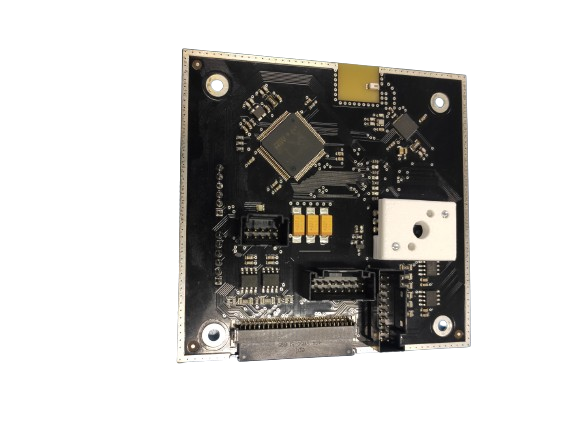
\includegraphics[scale=0.4]{images/radio-pcb}}
	\caption{Radio board of CVUT-SAT}
	\label{cvut-sat}
\end{figure}

The radio PCB is shown in the picture .... Is is composed of STM32F413 which can serve as a backup on board computer. This processor is connected via CAN bus with another chip nRF52832 which is capable of communication via Bluetooth Low Energy. The nRF processor is main subject of our interest because it is so to speak gateway of communication between Ground station and the cubesat.

\begin{figure}[htbp]
\centerline{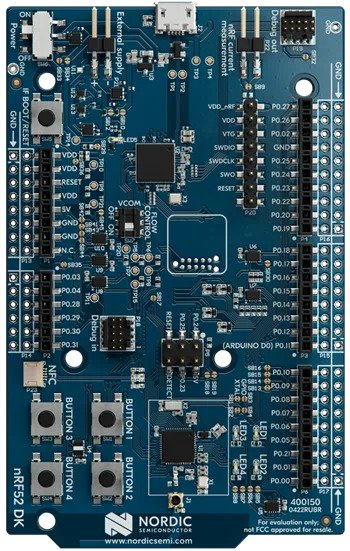
\includegraphics[scale=0.4]{images/nRF52-DK}}
\caption{nRF52 DK - Bluetooth Low Energy and Bluetooth mesh development kit for the nRF52810 and nRF52832 SoCs\cite{nrf-dk-shop}}
\label{nrfDK}
\end{figure}

Because for programming nRF52832 is needed programmer we have been given also nRF52 DK \cite{nrf-dk-shop} (development kit shown in the figure \ref{nrfDK}). The main part of this project was developed using this DK. Development kit contains debugger and also nRF52832. Debugger can be also used for emulating different nRF52 processors. On the kit there are 4 buttons and 4 LEDs so we can easily interact with the hardware.

The debugger on the development kit can be connected to the cubesat radio board using special programming jumper. Using that it is possible to program/debug also nRF chip on the board. STM32 processors commonly have proprietary bootloader which adds the possibility of downloading new firmware directly without using programmer. On the other hand you cannot debug the STM with this setup.

At the beginning of this report we will describe ISO/OSI model which is commonly known and used for describing communication protocols. Then we will introduce some communication protocols and then we describe Cubesat Space Protocol which we used in this project. Then we will describe Bluetooth. At the end we will describe laboratory part of our project. It means we propose our solution for the problem and we describe the provided code for the nRF and for the Ground station.

\section{OSI model}
The OSI model stands for Open Systems Interconnection model which serves as a foundational framework for understanding and designing communication protocols. It provides a systematic approach to conceptualizing and implementing network communication, ensuring interoperability between different systems. In 1983 OSI was adopted by the International Organization for Standardization (ISO) as ISO 7498, with the current version being ISO/IEC 7498-1:1994\cite{AWS-Amazon}. Since then it was adopted by all major computer and telecommunication companies. It was the first standard model for network communication. \cite{impreva-osi}

Because there many different incompatible machine technologies so this standard concept allows us to make agreement for how two different computer systems could exchange data. It helps visualize how digital communication operates. So before we dive deep into the space communication protocols we describe this OSI model. Then OSI model would be a good reference point. Beside of better understanding the space protocols OSI model is also aid in the development and evaluation of protocols.

The OSI model consists of seven abstract layers shown in the figure \ref{osi}. Each layer have specific purpose and functionality to perform. Each layer is independent and interacts directly with two other layers - layer above and bellow. But all layers work collaboratively and describes how the user/application data are transmitted. Using these layers we are allowed for more systematic approach to networking. Instead of having huge communication system, we are able to split it into these layers, each of which performs a specialized transmission function. \cite{geeks-osi}

\begin{figure}[htbp]
	\centerline{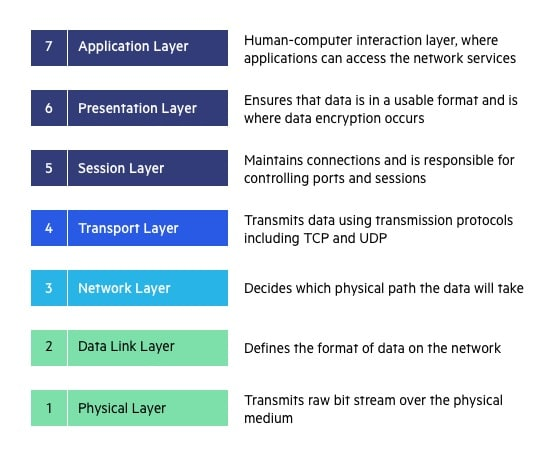
\includegraphics[scale=0.5]{images/OSI-7-layers}}
	\caption{Layers of the OSI model\cite{impreva-osi}}
	\label{osi}
\end{figure}

The precess of sending data using OSI is as follows: first, the sender application has to pass the data to the application layer which passes them down to the next lower layer. Then each layer adds its own headers before passing it on. The data communication moves down the layers until it is transmitted through the physical medium. Because OSI is only the abstraction, not every layer has to be present. At the other end of the medium each lazer processes the data according to the relevant headers.  The data moves up the layers and is gradually unpacked until the application layer of the receiver side.\cite{AWS-Amazon}

Now we are will shortly describe function of each layer \cite{impreva-osi, geeks-osi}.
\subsection{1 Physical layer}
Physical layer is the lowest layer. It encompassing the physical communication medium and the technologies involved in transmitting digital signals. It manages various channels like fiber-optic cables, copper cabling, and wireless connections, including standards like Bluetooth and Wi-Fi. This layer is crucial for establishing the actual cable or wireless link between network nodes, defining connectors, electrical cables, or wireless technologies. Its primary responsibility lies in transmitting raw data, consisting of 0s and 1s, while also overseeing bit rate control or a bit synchronization. The physical layer forms the foundation for the OSI model, handling the physical connections between devices and managing the transmission of individual bits between nodes. Upon receiving data, it converts the signal into 0s and 1s and forwards them to the Data Link layer for frame reconstruction.

\subsection{2 Data link layer}
The Data link layer, positioned above the physical layer in the OSI model, plays a crucial role in ensuring error-free node-to-node message delivery over the network. Divided into two sublayers, Logical Link Control (LLC) and Media Access Control (MAC), its primary functions include breaking up packets into frames, encapsulating MAC addresses in headers, and managing the connection between physically-connected nodes. When a packet arrives, the Data link layer uses the MAC address to transmit it to the host. This layer is responsible for tasks such as error checking, synchronization of frames, and defining permissions for data transmission and reception using MAC addresses. Ethernet is an example of a standard of this level.

\subsection{3 Network layer}
The Network layer focuses on routing, forwarding, and addressing within a distributed or interconnected network. It is breaking up segments into network so called packets. And it routs these packets by determining the optimal path across a physical network. It utilizes protocols like IPv4 and IPv6 for internet communication. Using network addresses, typically in the form of Internet Protocol (IP) addresses, it directs packets to their destination nodes. In the header, the sender and receiver's IP addresses are encapsulated by the network layer.

\subsection{4 Transport layer}
The Transport layer facilitates end-to-end delivery of messages, managing data in segments. It ensures proper transmission through segmentation, flow control, and error control. Transport layer also adds port numbers in it's header. This layer basically corresponds to the Transmission Control Protocol (TCP) or User Datagram Protocol (UDP). The TCP is near-lossless connection based protocol. On the other hand UDP is connectionless protocol, which is used for less critical applications.

\subsection{5 Session layer}
The Session layer establishes and manages communication connection (session) between devices, ensuring their functionality throughout data transfer. It handles connection establishment, session maintenance, authentication, and security. Protocols like Network File System (NFS) and Server Message Block (SMB) are commonly utilized at the session layer.

\subsection{6 Presentation layer}
The Presentation layer defines encoding, encryption, and compression methods to ensure accurate reception at the other end. This layer extracts and manipulates data from the application layer, adjusting it to the required format for network transmission. Example of used standards in this layer could be JSON, CSV or JPEG.

\subsection{7 Application layer}
Application layer is used by end-user. It provides protocols that allow software send and receive data. Examples of this layer protocols are HTTP which are used in web browsers of SMTP which is used by mail clients.

\subsection{Cubesat Space Protocol}
The Cubesat Space Protocol (CSP) is used as an transport and network layer of OSI model. It is based on TCP/IP which is older than OSI and less structured standard. CSP is a compact delivery protocol which was developed by students at Aalborg University in 2008. This protocol utilizes a 32-bit header containing both transport and network-layer information.\cite{Mineo-Wakita}

The protocol header contains source and destination addresses and basic means for authentication, encryption, establishing a connection and checksums. Since CSP is very slim other features require additional protocols.\cite{grillmayer}

The protocol allows define up to 32 addresses. The common topology is that addresses 0-15 are used on the space segment and the others are used in the ground system. It allows easy routing in the network.\cite{GomSpace}

Usage of CSP enables every subsystem to offer its services at the same network level, eliminating the need for any master node. Adopting a service-oriented architecture offers various advantages over the conventional master/slave topology. Namely authors of the protocol mentions these advantages: services maintain a relationship that minimizes dependencies between subsystems; reduces single point of failure; logic is divided into services with the intention of promoting reuse; beyond descriptions in the service contract, services hide logic from the outside world, etc. 

The implementation of the CSP is written in GNU C and can be compiled for FreeRTOS or Zephyr, which are real time operating systems or it can be compiled for Linux. Implementation is called Lib CSP.\cite{libcsp}

LibCSP incorporates two Transport Layer protocols: UDP (unreliable datagram protocol) and RDP (reliable datagram protocol). UDP operates as a datagram service, preserving data structures from entry to exit at the transport layer. The simplicity of UDP makes it practical for request/reply-based communication, especially in time-sensitive applications where dropped packets are preferable to delayed ones. However, UDP has limitations, particularly in larger file transfers, where automatic data acknowledgment becomes essential. To address this, the RDP protocol offers additional features like a three-way handshake, flow control, retransmission, and extended acknowledgment. These features enhance reliability and performance, making RDP suitable for scenarios where a more robust and controlled data transfer protocol is required.

CSP supports connection-less or connection oriented connections. To allocate a new connection we can use one of the provided functions: client connection (csp\_connect), open server soceket for listening (csp\_socket) or accept an incoming connection to the server (csp\_accept()).

There are also provided functions for sending, receiving CSP packets or for pinging.

The last main feature is routing table. Because the CSP is network protocol, if we want to route the packet to different location, we can configure routing table and enable routing.

As a data link layer there can be used various different interfaces such as AX.25 (KISS), CAN, I2C, etc. But the maximum transfer unit is based on the selected interface. For instance if you want to send larger packets over CAN interface which only allows a frame size of 8 bytes, then you have to use custom implementation of fragmentation protocol in the data link layer. Specifically for CAN there is already written a small protocol in the library.

\section{Bluetooth Low Energy}
Because we are supposed to establish the communication between nRF52 chip and the Ground station (PC) over the Bluetooth, we will now provide a description of Bluetooth Low Energy (BLE). BLE is a standard which is supported on the nRF52.

Bluetooth standard is managed bz a Bluetooth Special Interest Group (SIG). The most popular protocols nowadays are Bluetooth Classic and Bluetooth Low Energy. BLE targets markets where is demand for low power rather than throughput. BLE sends short bursts of data. Typically after the transmission the radio is going to the sleep state.\cite{NovelBits}

We will be using BLE as an data link layer or interface. So the need to firstly establish BLE connection which already implements whole OSI model - called BLE stack (fig. \ref{ble}). On the top of that we will run the CSP.

\begin{figure}[htbp]
	\centerline{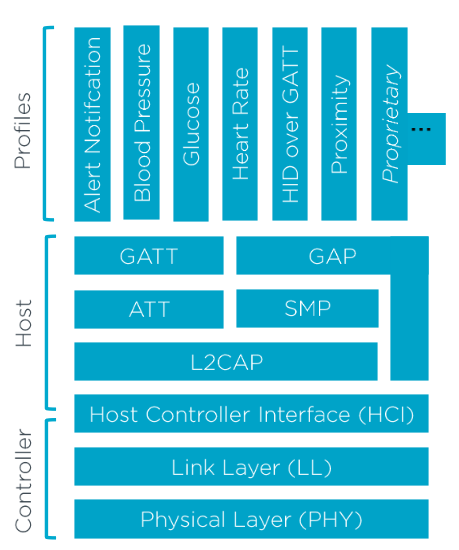
\includegraphics[scale=0.5]{images/ble-stack}}
	\caption{Bluetooth Low Energy protocol stack \cite{ble-nordic-intro}}
	\label{ble}
\end{figure}

The architecture of the BLE stack can be divided into three subsystems - controller, host and application.\cite{ble-nordic-intro}

The Controller contains physical layer which is 2.4 GHz ISM band. It can use one of 40 RF channels (2 MHz per each) with GFSK modulation. The link layer defines device address and manages packet format.

The Host contains Attribute Protocol (ATT). This layer provides client-server model - client device (typically phone/laptop) can access attributes on the server device (cubesat/IoT device). SMP layer is Security manager Protocol and it defines protocol for pairing and key distribution if you want to use secured BLE.
Another layer which is already interesting from developer point of view is GATT layer. GATT is highest data layer and uses ATT to discover and access attributes. GATT defines the format of the data exposed by a BLE device. GATT specifies structure of the attributes: services, characteristics and descriptors.

Services are grouping one or more attributes. Service should satisfy a specific functionality on the server. Each service provide characteristics which represents a piece of information that server wants to expose. Example of the service could be Heart Rate and it has characteristics Heart Rate Measurement and Body Sensor Location.

The last layer from the Host component is GAP. It is highest control layer - it defines how devices are discovered and connect to each other (so called advertisement). It also defines security modes.

On the top of that there are Profiles. Profile implements a specific application and it can be standard or proprietary. Most of the time the profiles are set by SIG. For instance there is standard The Heart Rate Profile which is used for medical and sport equipment. It consist of five also standardized services: The Generic Access Service, Generic Attribute Service, Battery Service, Device Information Service and Heart Rate Service. \cite{embeddedcentric}

\section{Laboratory part of the project}
Before you start you need to install few dependencies: libsocketcan, cmake, git, ninja-build.
\subsection{Modifications of libcsp}
We had to do some modifications of Lib CSP.

It would be handy to have an interface with only two functions - write and read. Write function should be called on demand from libcsp and calls Python's BLE send function. Read function should be called from the Python script when data over BLE is received. So we modified KISS interface, we got rid of the UART driver and provided only mentioned functions in the new interface.
 
We created new interface called basic which is located in libcsp/src/initerfaces/csp\_if\_basic.h. Corresponding header file is located in libcsp/include/csp/initerfaces/csp\_if\_basic.h. We also had to modify CMake file in libcsp/src/initerfaces/CMakeLists.txt.
The new provided interface contains basically these three functions:
\begin{enumerate}
	\item csp\_basic\_add\_interface - allocates and sets new interface (already working)
	\item csp\_basic\_tx - called by libcsp when it needs to send data over BLE (need to debug segfault)
	\item csp\_basic\_rx - called by Python to pass received packet to libcsp (need to create binding to Python)
\end{enumerate}

The last modified file is libcsp/src/bindings/python/pycsp.c which provides binding to Python. In this file we created pycsp\_basic\_init function which is binded to Python. Calling this you add new interface and you also pass a pointer to the Tx function which is stored in PyObject *py\_tx\_func. The fnc function is used to calling Python function stored in py\_tx\_func.

\subsection{nRF workspace installation procedure}
We are using nRF52832 DK as the development board. There are two available SDKs for this chip - nRF5 SDK which is in maintenance mode and it is not recommended to use it \cite{sdk}. The second SDK is called nRF Connect SDK \cite{connect} which is used in this project. It is based on Zephyr. It is real time operating system. Main advantage of using real time OS is that it allows us to create threads although we are using single core processor. It takes care about scheduling the threads. Fortunately, Zephyr is also OS that is natively supported by Lib CSP.

To use nRF Connect SDK you need to follow instructions from nRF Connect SDK docs.

Basically you need to install nRF Connect SDK extensions into your Visual Studio Code. You should use new Profile in the VS Code otherwise the standard extensions for developing C projects are going to be in conflict.

Then open installed extension and from that zou can download Toolchain. After that you should also download the SDK.

Now it is time to include Cubesat Space Protocol. Download the libcsp library. Now you should navigate to the ncs folder where the SDK has been downloaded (under Linux it should be in your home directory). Copy the libcsp library to the \lstinline{ncs/<sdk-version>/modules/lib} folder. Then you need to change \lstinline{ncs/<sdk-version>/nrf/west.yml} so open it and find the line with comment "Other third-party repositories". Under it add following two lines:
\begin{verbatim}
- name: libcsp
path: modules/lib/libcsp
\end{verbatim}

Then open folder nrf\_cubesat from the VS Code, now you need to create a new build. You need to choose the nrf52832dk\_nrf52832 profile. After that you can build the project and flash the code.

\subsection{nRF project}
In this project we are using unsecured connection. For the communication we are using Nordic UART Service (NUS). It is proprietary GATT service which allows as to asynchronously send byte array. We chose this service because there is no alternative defined by SIG. Implementation of NUS is already in the SDK. So it requires only correctly setup the BLE and we don't have to do any low level programming. In this service there are two characteristics: Rx and Tx. The main issue with this UART emulation over BLE is that we cannot send more than 20 bytes.

In the main file are two important functions. First of them is ble\_write\_thread which periodically sends data over BLE. Each 5 s it sends Hello World message with incrementing integer.

Second important function is bt\_receive\_cb which is called when data is received over BLE. Received data are printed into log and if received data is "1" it turns on LED3 or if received data is "0" it turns off LED3.

\subsection{Ground station workspace - installation procedure}
Project for the "Ground Station" is located in folder pc\_cubesat. First of all you have to install Python package called bleak which is package for controlling Bluetooth Low Energy. For the installation you can use provided requirements.txt file or run: pip3 install bleak.

\subsection{Ground station project}
In the project there are three Python files. First file example\_ble\_uart.py is compatible with nRF firmware which has been described above. It prints what nRF sends over NUS (Nordic UART Service) and periodically sends 1 or 0 to toggle the LED3 on the DK board.

The second file example\_csp\_server\_client.py is example file from the libcsp library. If you followed the installation procedure you should be able to run it. When the address is set to 0, it probably uses loopback interface.

Third file csp\_python\_binding.py is a script for testing of a new interface called basic which we created. This interface is based on KISS interface which has been already written in original library. KISS interface is a protocol used by hams and is used on top of the UART (thus works with serialized data).

The current struggle is with binding to Python. When you run the script, Python will pass pointer to the tx function. That pointer to the Python's function lives as an PyObject during initialization of the interface. Libcsp sucessfully calls the Tx function during initialization (row 232 in csp\_if\_basic.c) but when Python tries to send ping packet we will get a seg fault (row 27 in csp\_if\_basic.c). It is probably because of the freed memory on the address which is stored in py\_tx\_func.

\section{Conclusion}
In this report we described abstract OSI reference communication model. After that we described Cubesat Space Protocol and Bluetooth Low Energy. These protocols are used in our lab project. 

We managed to establish communication between nRF DK and the Ground Station (PC) using emulated UART over BLE. nRF runs on Zephyr and Ground Station is decoding packets received over BLE using Python script. We also learned how to compile CSP library on Zephyr - it is few simple steps, but these steps weren't well documented. We are also able to call Lib CSP functions from Python, because we set up bindings between Python. And last but not least we provided new simple interface called basic, which potentially can be used for direct data transfer between Lib CSP and our application.

We were unable to set up a binding between basic interface and Python. Therefore, we are not able to use CSP over BLE because we cannot call Python Tx function from the Lib CSP. The possible solution is to write the entire Ground Station in C (which includes controlling BLE in C). Or some expert on C-Python bindings could have solve this problem.

\section*{Acknowledgment}
We would like to thank the Space Engineering course team for lending us the hardware needed to create the work described here and for their advice on how to get started.

\bibliographystyle{unsrt}
\bibliography{bibliography}

\end{document}
